\documentclass[12pt,a4paper,twoside]{article}
\usepackage[utf8]{inputenc}
\usepackage{amsmath}
\usepackage{lmodern}
\usepackage{textcomp}
\usepackage{amsfonts}
\usepackage{amssymb}
\usepackage{graphicx}
\usepackage[left=2cm,right=2cm,top=2cm,bottom=2cm]{geometry}
\author{Carlos Eduardo Martínez Núñez}
% used in maketitle                                                             
\title{\textbf{Movimiento de la Tierra y la Luna Alrededor del Sol}}
\begin{document}
\maketitle
El presente estudio del movimiento de la tierra y la luna alrededor del sol, se centra en considerar el movimiento descrito por una trayectoria circular de la tierra respecto al sol, mientras la luna describe el mismo movimiento alrededor de la tierra. Para tal fin se considera a la tierra y la luna discribiendo una circunferencia al rededor del sol y la luna alrededor de la tierra, con un radio medio de R=1496000000 km, y r=149600000 km, respectivamente, como muestra la gráfica 1. 
\begin{figure}[htbp]
\centering
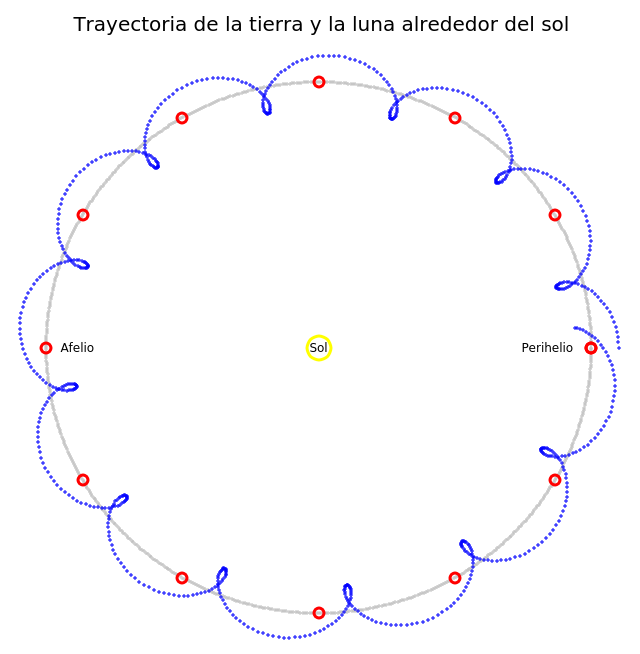
\includegraphics[width=12cm]{Trlunatierra.png}
\caption{Trayectoria de la tierra y la luna alrededor del sol.}\label{fig:figura1}
\end{figure}
La trayectoria de al tierra alrededor del sol, corresponde una una circunferencia descrita por la ecuación en coordenadas polares, dada como:
\begin{eqnarray}
R=1496000000
\end{eqnarray}
En termino de coordenadas cartesianas, esta trayectoria puede ser expresada por las ecuaciones:
\begin{eqnarray}
x_{t}=Rcos(\theta)\\
y_{t}=Rsin(\theta)
\end{eqnarray}
Donde $\theta$ corresponde al ángulo barrido por el radio de la tierra al sol.
La trayectoria de la luna respecto a la tierra, mientras la tierra se mueve, es el resultado de un movimiento relativo respecto al sol descrito por las ecuaciones:
\begin{eqnarray}
x_{_{l}}=Rcos(\theta)+rcos(\alpha)\\
y_{l}=Rsin(\theta)+rsin(\alpha)
\end{eqnarray}
Donde $\alpha$ corresponde al ángulo barrido por el radio de la luna a la tierra.
\section{Aplicación Fortran para el cálculo de la trayectoria de la la tierra alrededor del sol}
El código de la aplicación fortran para determinar la trayectoria en coordenadas cartesianas de la tierra y la luna alrededor del sol, corresponde a:
\begin{verbatim}
program tr_luna_tierra
!::::::::::::::::::::::::::::::::::::::::::::::::::::::::::::::::::::::::::::::::::::
  !Aplicación Fortran para calcular la trayectoria de la luna respecto a la posicion
  !de la tierra alrededor del sol
  !al rededor del sol
  !r------------radio medio de la tierra al sol
  !xt------------Abcisa (coordenadas cartesianas)
  !yt------------Ordenada (Coordenadas cartesianas)
  !xl------------Abcisa de la luna respecto a la tierra
  !yl------------Ordenada de la luna respecto a la tierra
  !angle_a-------ángulo barrido por la tierra
  !angle_b-------ángulo barrido por la luna
  !Tl------------Periodo de la luna en seg
  !Tt------------Periodo de la tierra en seg
!::::::::::::::::::::::::::::::::::::::::::::::::::::::::::::::::::::::::::::::::::::
  implicit none
  integer, parameter::t=8766
  integer:: i
  double precision, parameter:: pi=3.141592d0,  Tt=8.766d3, Tl=6.56d2
  double precision::x_t, y_t, x_l, y_l
  double precision::ang_a, ang_b
  double precision,dimension(0:t)::xt2, yt2, xl2, yl2,dt
   
 
     !Making file to storage data
    open (1,file="tr_luna_tierra.txt",status="unknown") 
    
     !loop to calculate trayectory
    do i=0,t,12
       !angulo en radianes
     dt(i)=dble(i)
     ang_a=(dt(i)*2.0d0*pi)/Tt
     ang_b=(dt(i)*2.0d0*pi)/Tl
     !Calling  subroutine
    call tr_luna (ang_a,ang_b,x_t,y_t,x_l,y_l)
   
    xt2(i)=x_t
    yt2(i)=y_t
    xl2(i)=x_l
    yl2(i)=y_l
   
     !Saving data
       write (1,*) xt2(i), yt2(i), xl2(i), yl2(i)
    end do
      close(1)
 end program tr_luna_tierra

!:::::::::::::::::::::::::::::::::::::::::::::::::::::::::::::::::::::::::::::::

subroutine tr_luna (angle_a,angle_b,xt,yt,xl,yl)
  implicit none
   
   double precision,intent(in)::angle_a, angle_b
   double precision, intent(out)::xt, yt, xl, yl
   double precision, parameter :: Rt=1.496d8, Rl=1.496d7 !radio de la tierray luna

     !procesing  data 
    xt=Rt*dcos(angle_a)
    yt=Rt*dsin(angle_a)
    xl=Rt*dcos(angle_a)+Rl*dcos(angle_b)
    yl=Rt*dsin(angle_a)+Rl*dsin(angle_b)


    end subroutine tr_luna

\end{verbatim}
El Scritp para la graficación de los datos de salida usando Gnuplot corresponde a:
\begin{verbatim}
set title "Trayectoria de la tierra y la luna alrededor del sol"
set title font ",15" norotate
set style data lines
set style data points
set pointsize 0.5
unset key
unset border
unset xtics
unset ytics
set xrange [-165023000:165023000]
set yrange [-165023000:165023000]
set label 1 "Sol" at 0.0,0.0 center front
set label 2 "Perihelio" at 111600000.00000000, 0.0000000000000000
set label 3 "Afelio" at -141599999.99996805, 97.777033044205780
plot "tr_luna_tierra.txt" using 1:2 ls 1 lw 1 lc rgb "gray",\
"tr_luna_tierra.txt" using 3:4 ls 1 lw 1 lc rgb "blue",\
"pst_tierra.txt" using 1:2 ls 6 lw 10 lc rgb "red",\
"center.txt" using 1:2 ls 6 lw 24 lc rgb "yellow"
\end{verbatim}
\end{document}